
\documentclass[11pt,a4paper]{article}

\usepackage[margin=0.85in]{geometry}
\usepackage{amsmath}
\usepackage{booktabs}
\usepackage{longtable}
\usepackage{array}
\usepackage{enumitem}
\usepackage{xcolor}
\usepackage{hyperref}
\usepackage{listings}
\usepackage{tikz}
\usepackage{fancyhdr}
\usetikzlibrary{arrows.meta,positioning,shapes.geometric,fit}

\hypersetup{colorlinks=true,linkcolor=blue,urlcolor=blue}
\setlist[itemize]{leftmargin=1.5em}
\setlist[enumerate]{leftmargin=1.7em}

\lstdefinestyle{manual}{
  basicstyle=\ttfamily\small,
  breaklines=true,
  frame=single,
  columns=fullflexible
}
\lstset{style=manual}

\pagestyle{fancy}\fancyhf{}
\fancyhead[L]{Agentic AI Bootcamp}
\fancyhead[R]{sujeet.banerjee@gmail.com\\sujeet.banerjee.professional@gmail.com}
\fancyfoot[L]{Graph-RAG, Knw-Graphs}
\fancyfoot[R]{\thepage}


\title{\textbf{Advanced RAG: Graph-RAG Architecture}\\
\large Reference Manual: Knowledge Graphs and Graph-Aware Inference}
\author{Sujeet Banerjee}
\date{}

\begin{document}
\maketitle
\tableofcontents
\newpage

\section{Purpose and Scope}

Graph-RAG combines semantic retrieval from vector representations with explicit relationship retrieval from a graph-based knowledge representation. The architecture is intended to address questions whose answers depend not only on locating relevant passages, but also on identifying relationships, dependencies, paths, impacts, or multi-hop connections between entities.

A conventional Retrieval-Augmented Generation pipeline is commonly represented as:

\begin{center}
\texttt{Query $\rightarrow$ Embedding $\rightarrow$ Vector Search $\rightarrow$ Top-K Chunks $\rightarrow$ LLM}
\end{center}

A Graph-RAG architecture introduces an additional knowledge representation:

\begin{center}
\texttt{Documents $\rightarrow$ Chunks $\rightarrow$ VectorDB}\\
\texttt{Documents $\rightarrow$ Entities + Relationships $\rightarrow$ GraphDB}
\end{center}

At inference time, the retrieval system may combine semantic relevance with graph structure:

\begin{center}
\texttt{Query $\rightarrow$ Vector Retrieval + Graph Retrieval $\rightarrow$ Candidate Fusion $\rightarrow$ Reranking $\rightarrow$ Context Construction $\rightarrow$ LLM}
\end{center}

Graph-RAG is not a single fixed implementation pattern. The graph may influence retrieval before vector search, after vector search, in parallel with vector search, or primarily during context construction.

\section{Core Data Representations}

\subsection{Document Chunks}

A source document is divided into chunks suitable for embedding and retrieval.

Example:

\begin{lstlisting}
Chunk C1:
Order Service calls Payment Service.

Chunk C2:
Payment Service uses Payments DB.

Chunk C3:
Checkout depends on Order Service.
\end{lstlisting}

Each chunk normally receives a stable identifier:

\begin{lstlisting}
chunk_id = C1
document_id = architecture_doc_01
\end{lstlisting}

The chunk identifier is important because it can provide provenance and linkage between vector evidence and graph entities.

\subsection{Entities}

Entities represent domain-specific objects.

Example entity types:

\begin{lstlisting}
Service
Database
API
Incident
Team
CustomerFeature
\end{lstlisting}

Example entities:

\begin{lstlisting}
Order Service
Payment Service
Payments DB
Checkout
INC-102
\end{lstlisting}

Entities should normally have stable canonical identifiers:

\begin{lstlisting}
service_order
service_payment
database_payments
feature_checkout
incident_102
\end{lstlisting}

\subsection{Relationships}

Relationships represent explicit domain connections.

Example:

\begin{lstlisting}
Order Service --CALLS--> Payment Service
Payment Service --USES--> Payments DB
Order Service --SUPPORTS--> Checkout
INC-102 --AFFECTED--> Payment Service
\end{lstlisting}

The graph may be represented conceptually as:

\begin{center}
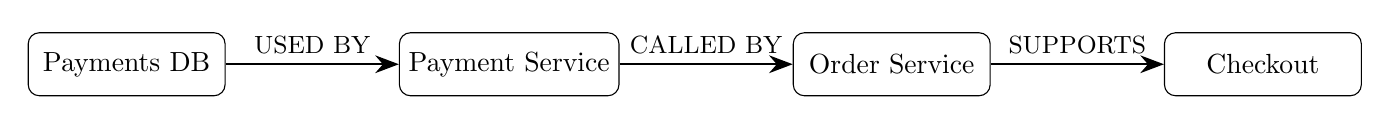
\begin{tikzpicture}[
node distance=2.2cm,
box/.style={draw,rounded corners,minimum width=2.5cm,minimum height=.8cm,align=center},
arrow/.style={-{Stealth[length=3mm]},thick}
]
\node[box] (db) {Payments DB};
\node[box,right=of db] (pay) {Payment Service};
\node[box,right=of pay] (order) {Order Service};
\node[box,right=of order] (checkout) {Checkout};
\draw[arrow] (db) -- node[above,font=\small]{USED BY} (pay);
\draw[arrow] (pay) -- node[above,font=\small]{CALLED BY} (order);
\draw[arrow] (order) -- node[above,font=\small]{SUPPORTS} (checkout);
\end{tikzpicture}
\end{center}

\section{Ontology, Extraction Rulebook, and Graph Facts}

Three concepts should remain separate.

\subsection{Ontology or Schema}

The ontology defines what kinds of entities and relationships are valid.

Example:

\begin{lstlisting}
Entities:
- Service
- Database
- Incident

Relationships:
- USES
- CALLS
- DEPENDS_ON
- AFFECTED
\end{lstlisting}

A schema may define valid source and target types:

\begin{center}
\texttt{Service --USES--> Database}
\end{center}

The schema answers:

\begin{quote}
What entities and relationships are permitted in the knowledge model?
\end{quote}

\subsection{Extraction Rulebook}

The extraction rulebook defines how text should be interpreted when identifying relationships.

Example:

\begin{lstlisting}
USES:
A Service uses a Database when the source explicitly
states that the Service reads from, writes to, stores
data in, retrieves data from, or persists data to the
Database.

CALLS:
A Service calls another Service when the source
explicitly states that it invokes an API, endpoint,
RPC interface, or synchronous service request.
\end{lstlisting}

The rulebook answers:

\begin{quote}
How should textual evidence be interpreted as a graph relationship?
\end{quote}

\subsection{Graph Facts}

Graph facts are the extracted and validated results.

\begin{lstlisting}
(Payment Service)-[:USES]->(Payments DB)

(Order Service)-[:CALLS]->(Payment Service)
\end{lstlisting}

The graph answers:

\begin{quote}
What relationships are represented as facts in the knowledge base?
\end{quote}

\subsection{Recommended Storage Separation}

A practical architecture is:

\begin{center}
\texttt{Git / Configuration Repository}\\
$\downarrow$\\
\texttt{Ontology + Extraction Rules}\\
$\downarrow$\\
\texttt{Extraction and Validation Pipeline}\\
$\downarrow$\\
\texttt{Graph Database}
\end{center}

The GraphDB primarily stores extracted facts, entities, relationships, and provenance. The complete extraction rulebook does not need to be stored in the GraphDB.

A rule version may nevertheless be recorded as provenance:

\begin{lstlisting}
(Payment Service)-[:USES {
  confidence: 0.94,
  extractor_version: "graph-extractor-v2",
  ontology_version: "1.3",
  rule_version: "2.1",
  source_chunk_id: "C2"
}]->(Payments DB)
\end{lstlisting}

\section{Ingestion Architecture}

A complete ingestion pipeline can be represented as:

\begin{center}
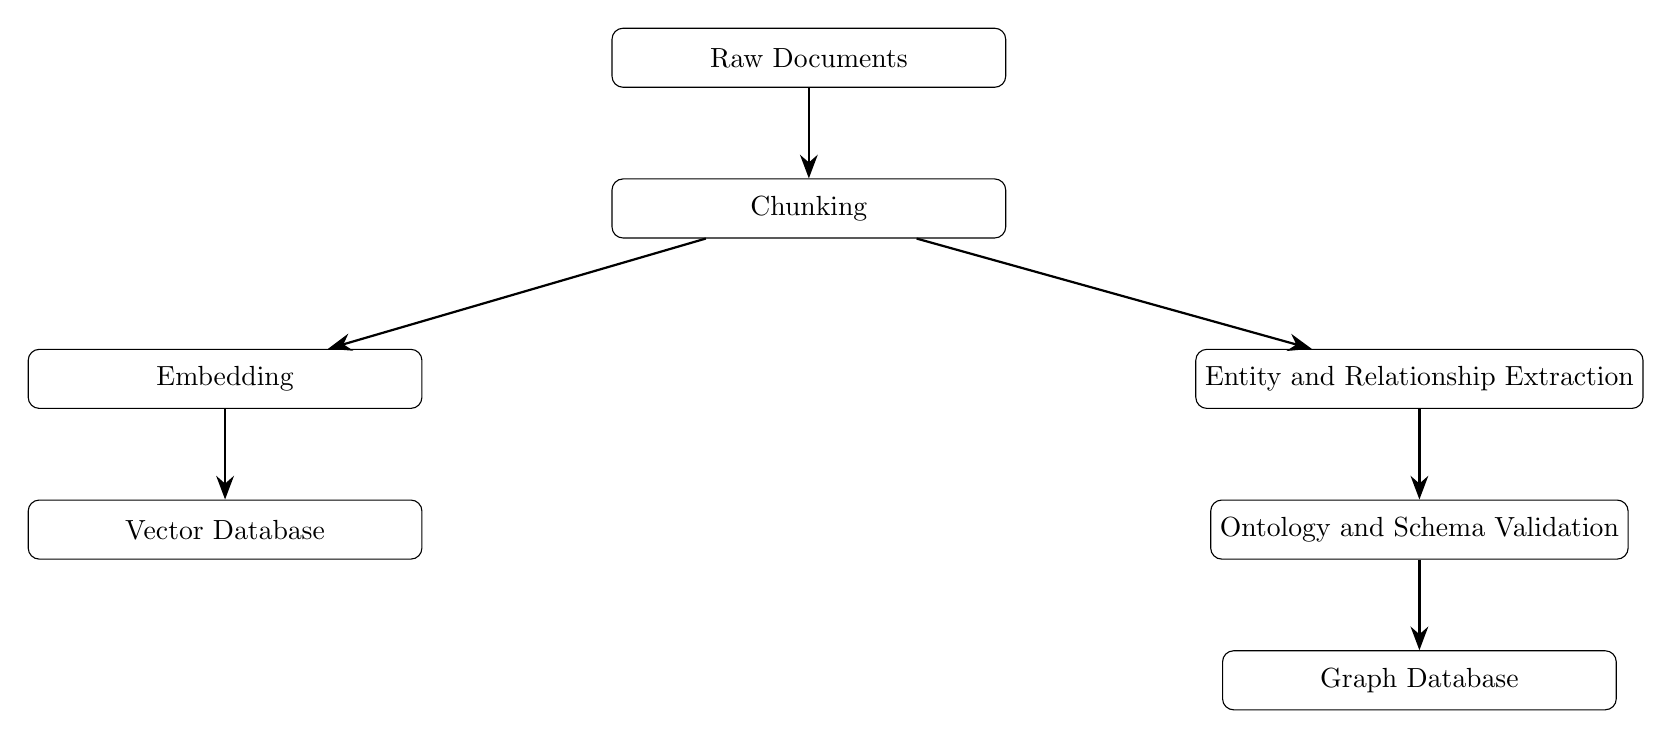
\begin{tikzpicture}[
node distance=1.15cm,
box/.style={draw,rounded corners,minimum width=5cm,minimum height=.75cm,align=center},
arrow/.style={-{Stealth[length=3mm]},thick}
]
\node[box] (doc) {Raw Documents};
\node[box,below=of doc] (chunk) {Chunking};
\node[box,below left=1.4cm and 2.4cm of chunk] (embed) {Embedding};
\node[box,below=of embed] (vector) {Vector Database};
\node[box,below right=1.4cm and 2.4cm of chunk] (extract) {Entity and Relationship Extraction};
\node[box,below=of extract] (validate) {Ontology and Schema Validation};
\node[box,below=of validate] (graph) {Graph Database};
\draw[arrow] (doc)--(chunk);
\draw[arrow] (chunk)--(embed);
\draw[arrow] (embed)--(vector);
\draw[arrow] (chunk)--(extract);
\draw[arrow] (extract)--(validate);
\draw[arrow] (validate)--(graph);
\end{tikzpicture}
\end{center}

\subsection{Vector Storage}

The original or normalized chunk text is embedded:

\begin{lstlisting}
"Payment Service uses Payments DB."
        |
        v
Embedding Model
        |
        v
Vector
\end{lstlisting}

The vector store may contain:

\begin{lstlisting}
vector: [0.012, -0.442, ...]
chunk_id: C2
document_id: architecture_doc_01
entity_ids:
  - service_payment
  - database_payments
\end{lstlisting}

\subsection{Graph Storage}

The graph extraction branch stores:

\begin{lstlisting}
(service_payment)-[:USES]->(database_payments)
\end{lstlisting}

The same entity identifiers provide a logical bridge:

\begin{center}
\begin{tabular}{lll}
\toprule
GraphDB & Shared Identifier & VectorDB \\
\midrule
Payment Service & service\_payment & Chunks mentioning service\_payment \\
Payments DB & database\_payments & Chunks mentioning database\_payments \\
\bottomrule
\end{tabular}
\end{center}

\section{Should Chunks Be Enriched Before Vectorization?}

There are several valid patterns.

\subsection{Pattern A: Minimal Enrichment}

The original chunk is embedded without graph expansion.

Example metadata:

\begin{lstlisting}
{
  "chunk_id": "C2",
  "document_id": "architecture_doc_01",
  "entity_ids": [
    "service_payment",
    "database_payments"
  ]
}
\end{lstlisting}

Advantages include separation between local source evidence and global graph structure. A change to the graph does not automatically require regeneration of all affected embeddings.

This pattern is a suitable default implementation.

\subsection{Pattern B: Graph Metadata Enrichment}

Graph-derived information may be attached as metadata:

\begin{lstlisting}
{
  "chunk_id": "C2",
  "entities": [
    "Payment Service",
    "Payments DB"
  ],
  "relationships": [
    "Payment Service USES Payments DB"
  ],
  "related_entities": [
    "Order Service",
    "Checkout"
  ]
}
\end{lstlisting}

The metadata can support filtering and candidate generation.

\subsection{Pattern C: Embed Graph-Expanded Text}

The original chunk may be augmented with additional graph-derived context before embedding.

Example:

\begin{lstlisting}
Original:
Payment Service uses Payments DB.

Expanded:
Payment Service uses Payments DB.
Order Service calls Payment Service.
Order Service supports Checkout.
\end{lstlisting}

This approach should be used carefully. Graph-expanded text can blur the distinction between source evidence and derived knowledge. Graph changes may also require re-embedding previously generated vectors.

For most implementations, explicit graph traversal at retrieval time is preferable to indiscriminate expansion of chunk text before embedding.

\section{The Link Between VectorDB and GraphDB}

The relationship between graph evidence and vector evidence is usually not a relational database join based on vector similarity.

The common architecture is based on stable identifiers and provenance.

Example:

\begin{lstlisting}
Graph:
(Payment Service {id: S1})
    -[:USES]->
(Payments DB {id: D1})

Vector metadata:
Chunk C2
entity_ids = [S1, D1]
\end{lstlisting}

The retrieval layer can therefore answer:

\begin{quote}
Which chunks provide textual evidence for this graph node or graph path?
\end{quote}

This may be implemented through:

\begin{itemize}
\item entity IDs stored in vector metadata;
\item chunk IDs stored as node or relationship provenance;
\item an external entity-to-chunk index;
\item a document provenance table;
\item a unified retrieval system supporting both graph and vector operations.
\end{itemize}

\section{Inference Architecture}

Consider the query:

\begin{quote}
\textbf{What happens to Checkout if Payments DB fails?}
\end{quote}

A hybrid inference architecture can perform parallel retrieval.

\begin{center}
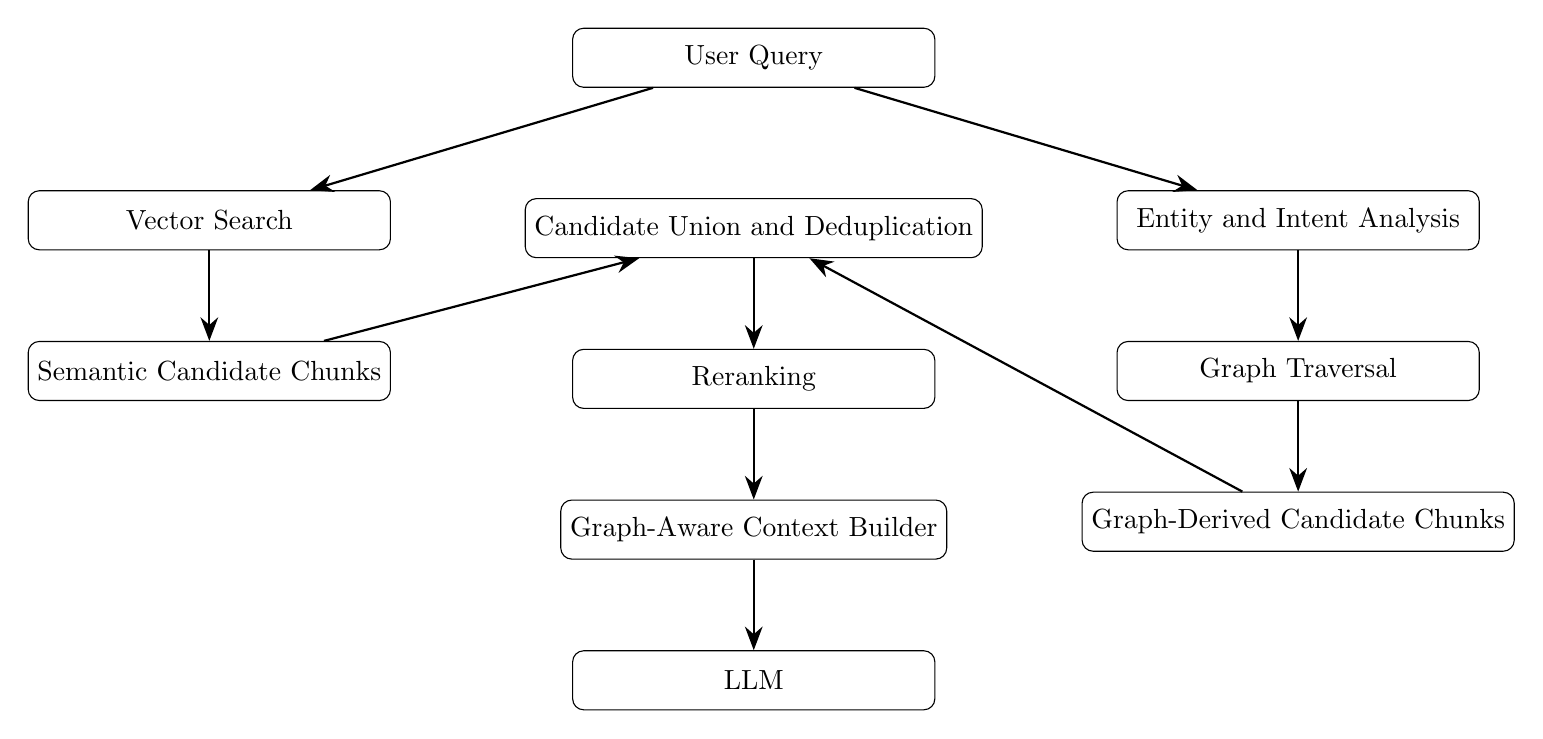
\begin{tikzpicture}[
node distance=1.15cm,
box/.style={draw,rounded corners,minimum width=4.6cm,minimum height=.75cm,align=center},
arrow/.style={-{Stealth[length=3mm]},thick}
]
\node[box] (query) {User Query};
\node[box,below left=1.3cm and 2.3cm of query] (vs) {Vector Search};
\node[box,below right=1.3cm and 2.3cm of query] (entity) {Entity and Intent Analysis};
\node[box,below=of vs] (vc) {Semantic Candidate Chunks};
\node[box,below=of entity] (gs) {Graph Traversal};
\node[box,below=of gs] (gc) {Graph-Derived Candidate Chunks};
\node[box,below=1.4cm of query] (fusion) {Candidate Union and Deduplication};
\node[box,below=of fusion] (rerank) {Reranking};
\node[box,below=of rerank] (context) {Graph-Aware Context Builder};
\node[box,below=of context] (llm) {LLM};
\draw[arrow] (query)--(vs);
\draw[arrow] (query)--(entity);
\draw[arrow] (vs)--(vc);
\draw[arrow] (entity)--(gs);
\draw[arrow] (gs)--(gc);
\draw[arrow] (vc)--(fusion);
\draw[arrow] (gc)--(fusion);
\draw[arrow] (fusion)--(rerank);
\draw[arrow] (rerank)--(context);
\draw[arrow] (context)--(llm);
\end{tikzpicture}
\end{center}

\section{Vector Retrieval Branch}

The query is embedded:

\begin{lstlisting}
"What happens to Checkout if Payments DB fails?"
                    |
                    v
             Query Embedding
                    |
                    v
               Vector Search
\end{lstlisting}

Example results:

\begin{center}
\begin{tabular}{llr}
\toprule
Chunk & Content & Similarity \\
\midrule
C2 & Payment Service uses Payments DB. & 0.91 \\
C8 & A database outage caused payment authorization failures. & 0.85 \\
C12 & Checkout requires successful payment authorization. & 0.79 \\
\bottomrule
\end{tabular}
\end{center}

The vector branch answers:

\begin{quote}
Which passages are semantically similar to the query?
\end{quote}

It does not inherently guarantee that all intermediate dependencies required for an impact analysis are retrieved.

\section{Graph Retrieval Branch}

The query is analyzed for known entities and intent.

Example:

\begin{lstlisting}
Entity:
Payments DB

Intent:
Impact analysis

Target:
Checkout
\end{lstlisting}

Graph traversal can identify a dependency path:

\begin{center}
\texttt{Payments DB}\\
$\downarrow$ \texttt{USED BY}\\
\texttt{Payment Service}\\
$\downarrow$ \texttt{CALLED BY}\\
\texttt{Order Service}\\
$\downarrow$ \texttt{SUPPORTS}\\
\texttt{Checkout}
\end{center}

The relevant entity set is:

\begin{lstlisting}
database_payments
service_payment
service_order
feature_checkout
\end{lstlisting}

The retrieval layer then maps these entities to supporting chunks.

Example:

\begin{center}
\begin{tabular}{ll}
\toprule
Entity & Associated Chunks \\
\midrule
Payments DB & C2, C8 \\
Payment Service & C2, C5, C8 \\
Order Service & C3, C9 \\
Checkout & C12, C14 \\
\bottomrule
\end{tabular}
\end{center}

The graph-derived candidate set may therefore be:

\begin{lstlisting}
C2
C3
C5
C8
C9
C12
C14
\end{lstlisting}

\section{Candidate Fusion}

The vector and graph branches generate partially overlapping evidence.

Example:

\begin{lstlisting}
Vector candidates:
C2, C8, C12

Graph-derived candidates:
C2, C3, C5, C8, C9, C12, C14
\end{lstlisting}

The union is:

\begin{lstlisting}
C2, C3, C5, C8, C9, C12, C14
\end{lstlisting}

This process is better described as \textbf{candidate generation and candidate fusion} than as a traditional database join.

\section{Candidate Scoring and Reranking}

A manual hybrid score may be defined as:

\[
Score(c) =
\alpha S_v(c) +
\beta S_g(c) +
\gamma S_e(c) +
\delta S_m(c)
\]

where:

\begin{itemize}
\item $S_v(c)$ is vector semantic similarity;
\item $S_g(c)$ is graph relevance, such as path proximity;
\item $S_e(c)$ is entity overlap with the query or relevant subgraph;
\item $S_m(c)$ is additional metadata relevance.
\end{itemize}

Example:

\[
Score(c) =
0.5 \times SemanticSimilarity +
0.3 \times GraphRelevance +
0.2 \times EntityMatch
\]

An alternative is to use a reranker.

The reranker receives:

\begin{lstlisting}
Query
+
Candidate chunks from vector retrieval
+
Candidate chunks from graph retrieval
\end{lstlisting}

It produces a relevance ordering based on the complete query and candidate content.

This architecture avoids forcing all graph and semantic signals into a manually designed formula.

\section{Graph-Guided Vector Retrieval}

Graph information can also be used before vector ranking.

The process is:

\begin{center}
\texttt{Query}\\
$\downarrow$\\
\texttt{Entity Extraction}\\
$\downarrow$\\
\texttt{Graph Traversal}\\
$\downarrow$\\
\texttt{Relevant Entity IDs}\\
$\downarrow$\\
\texttt{Vector Search Restricted to Relevant Entity Neighborhood}\\
$\downarrow$\\
\texttt{Semantic Ranking}
\end{center}

Example vector query conceptually:

\begin{lstlisting}
Search vectors where:

entity_id IN [
  service_payment,
  service_order,
  feature_checkout
]

ORDER BY semantic similarity
\end{lstlisting}

This creates a two-stage relevance mechanism:

\begin{enumerate}
\item The graph identifies the structurally relevant knowledge neighborhood.
\item The vector store identifies the most semantically relevant evidence within that neighborhood.
\end{enumerate}

\section{Retrieval Strategies}

\subsection{Vector-First}

\begin{center}
\texttt{Query $\rightarrow$ Vector Search $\rightarrow$ Retrieved Chunks $\rightarrow$ Entity Identification $\rightarrow$ Graph Expansion}
\end{center}

This pattern is useful when the query does not clearly identify a graph node.

Example:

\begin{quote}
What are the major risks during payment processing?
\end{quote}

Semantic retrieval can identify candidate entities before graph traversal.

\subsection{Graph-First}

\begin{center}
\texttt{Query $\rightarrow$ Entity Extraction $\rightarrow$ Graph Traversal $\rightarrow$ Entity Neighborhood $\rightarrow$ Filtered Vector Search}
\end{center}

This pattern is suitable when the query contains a clear entity.

Example:

\begin{quote}
What happens if Payments DB fails?
\end{quote}

\subsection{Parallel Hybrid Retrieval}

\begin{center}
\texttt{Query}\\
$\swarrow \hspace{3cm} \searrow$\\
\texttt{Vector Search \hspace{1cm} Graph Search}\\
$\downarrow \hspace{4cm} \downarrow$\\
\texttt{Candidate Fusion}\\
$\downarrow$\\
\texttt{Reranking}\\
$\downarrow$\\
\texttt{Context Construction}\\
$\downarrow$\\
\texttt{LLM}
\end{center}

This pattern is a suitable general-purpose architecture because neither retrieval mechanism is required to be perfect independently.

\section{Graph-Aware Context Construction}

The final context should not necessarily consist only of concatenated chunks.

A structured context can include both the graph path and the textual evidence.

Example:

\begin{lstlisting}
USER QUESTION:
What happens to Checkout if Payments DB fails?

DEPENDENCY PATH:

Payments DB
  -> USED BY
Payment Service
  -> CALLED BY
Order Service
  -> SUPPORTS
Checkout

SUPPORTING EVIDENCE:

[C2]
Payment Service uses Payments DB.

[C4]
Order Service calls Payment Service during checkout.

[C7]
Order Service supports Checkout.

[Historical Evidence]
A previous Payments DB outage caused payment
authorization failures.
\end{lstlisting}

The LLM receives:

\begin{enumerate}
\item explicit structural relationships;
\item source-backed textual evidence;
\item optionally ranked historical or operational evidence.
\end{enumerate}

The graph path should normally remain traceable to the underlying source evidence.

\section{End-to-End Worked Example}

Consider the source material:

\begin{quote}
Payment Service stores transaction records in Payments DB. Order Service calls Payment Service during checkout. Checkout requires successful payment authorization.
\end{quote}

\subsection{Step 1: Chunking}

\begin{lstlisting}
C1:
Payment Service stores transaction records in Payments DB.

C2:
Order Service calls Payment Service during checkout.

C3:
Checkout requires successful payment authorization.
\end{lstlisting}

\subsection{Step 2: Entity Extraction}

\begin{lstlisting}
Payment Service -> Service
Payments DB -> Database
Order Service -> Service
Checkout -> CustomerFeature
\end{lstlisting}

\subsection{Step 3: Relationship Extraction}

The rulebook maps textual evidence to relationships:

\begin{lstlisting}
"stores transaction records in"
    =>
Payment Service --USES--> Payments DB

"calls"
    =>
Order Service --CALLS--> Payment Service

"requires successful payment authorization"
    =>
Checkout --DEPENDS_ON--> Payment Authorization
\end{lstlisting}

Additional domain modeling may connect payment authorization to Payment Service.

\subsection{Step 4: Graph Validation}

Examples:

\begin{lstlisting}
Service --USES--> Database             VALID
Service --CALLS--> Service             VALID
CustomerFeature --DEPENDS_ON--> API    VALID
\end{lstlisting}

Invalid relationships are rejected or sent for review.

\subsection{Step 5: Vectorization}

Each source chunk is embedded independently.

Metadata:

\begin{lstlisting}
C1:
entity_ids = [service_payment, database_payments]

C2:
entity_ids = [service_order, service_payment]

C3:
entity_ids = [feature_checkout, service_payment]
\end{lstlisting}

\subsection{Step 6: User Query}

\begin{quote}
If Payments DB becomes unavailable, what is the likely impact on Checkout?
\end{quote}

\subsection{Step 7: Plain RAG Retrieval}

Plain vector search may retrieve:

\begin{lstlisting}
C1:
Payment Service stores transaction records in Payments DB.

C3:
Checkout requires successful payment authorization.
\end{lstlisting}

The intermediate dependency through Payment Service and Order Service may not be retrieved if similarity scoring does not rank the required passage highly enough.

\subsection{Step 8: Graph-RAG Retrieval}

Graph traversal identifies:

\begin{center}
\texttt{Payments DB}\\
$\downarrow$\\
\texttt{Payment Service}\\
$\downarrow$\\
\texttt{Order Service}\\
$\downarrow$\\
\texttt{Checkout}
\end{center}

The graph-derived entity set is used to retrieve supporting chunks:

\begin{lstlisting}
C1: Payment Service <-> Payments DB
C2: Order Service <-> Payment Service
C3: Checkout <-> Payment Service
\end{lstlisting}

The final context contains the complete dependency chain and supporting evidence.

\section{Advantages Over Plain RAG}

\begin{longtable}{p{3.2cm}p{5.5cm}p{5.5cm}}
\toprule
Capability & Plain RAG & Graph-RAG \\
\midrule
\endhead
Primary retrieval signal & Semantic similarity & Semantic similarity plus graph structure \\
Multi-hop dependencies & Incidental & Explicit graph traversal \\
Known entity relationships & Usually implicit in text & Explicitly represented \\
Impact analysis & Depends on retrieving all relevant chunks & Can traverse dependency paths \\
Candidate expansion & Primarily Top-K similarity & Graph neighborhood expansion \\
Retrieval filtering & Metadata and similarity filters & Entity, path, neighborhood, and relationship filters \\
Context structure & Usually chunk concatenation & Chunks plus explicit graph paths \\
Explainability & Passage-level evidence & Passage-level evidence plus relationship provenance \\
\bottomrule
\end{longtable}

\section{Reference Implementation Plan}

\subsection{Phase 1: Plain RAG Baseline}

Implement:

\begin{enumerate}
\item document ingestion;
\item chunking;
\item embedding generation;
\item VectorDB storage;
\item Top-K similarity retrieval;
\item reranking, if required;
\item context assembly;
\item LLM answer generation.
\end{enumerate}

Record baseline metrics for retrieval quality and answer quality.

\subsection{Phase 2: Entity and Relationship Extraction}

Implement:

\begin{enumerate}
\item domain ontology;
\item extraction rulebook;
\item entity extraction;
\item entity normalization and resolution;
\item relationship extraction;
\item confidence generation;
\item schema validation;
\item source provenance capture.
\end{enumerate}

Recommended configuration layout:

\begin{lstlisting}
project/
|
+-- schemas/
|   +-- graph_schema.yaml
|
+-- rules/
|   +-- relationship_rules.yaml
|
+-- ingestion/
|   +-- chunking.py
|   +-- entity_extraction.py
|   +-- relationship_extraction.py
|
+-- retrieval/
|   +-- vector_retriever.py
|   +-- graph_retriever.py
|   +-- fusion.py
|   +-- reranker.py
|
+-- evaluation/
    +-- datasets/
    +-- graph_rag_eval.py
\end{lstlisting}

\subsection{Phase 3: Graph Storage and Provenance}

Create graph nodes and relationships.

Store provenance:

\begin{lstlisting}
entity_id
relationship_type
source_chunk_id
source_document_id
confidence
extractor_version
ontology_version
rule_version
created_at
\end{lstlisting}

\subsection{Phase 4: Cross-Store Linkage}

Ensure that chunks and graph facts can be connected.

Recommended linkage:

\begin{lstlisting}
Vector chunk
  -> chunk_id
  -> entity_ids

Graph node
  -> entity_id

Graph relationship
  -> source_chunk_ids
\end{lstlisting}

This enables both directions:

\begin{center}
\texttt{Entity $\rightarrow$ Supporting Chunks}
\end{center}

and

\begin{center}
\texttt{Chunk $\rightarrow$ Mentioned Entities $\rightarrow$ Graph Neighborhood}
\end{center}

\subsection{Phase 5: Parallel Retrieval}

Implement:

\begin{enumerate}
\item semantic vector retrieval;
\item query entity extraction;
\item graph entity resolution;
\item graph traversal;
\item graph-to-chunk mapping;
\item candidate union;
\item deduplication.
\end{enumerate}

\subsection{Phase 6: Candidate Reranking}

Provide the reranker with:

\begin{lstlisting}
Query

Candidate source:
- vector
- graph
- both

Chunk content

Optional graph relevance:
- hop distance
- path membership
- entity overlap
\end{lstlisting}

Compare:

\begin{enumerate}
\item vector-only ranking;
\item graph-only candidate generation;
\item hybrid candidate fusion;
\item hybrid candidate fusion plus reranking.
\end{enumerate}

\subsection{Phase 7: Graph-Aware Context Builder}

Construct context using sections such as:

\begin{lstlisting}
Question

Relevant entities

Relationship path

Supporting source evidence

Optional contradictory evidence

Instructions for evidence-grounded answer generation
\end{lstlisting}

The context builder should enforce token budgets and avoid including graph information that cannot be traced to an approved or validated knowledge source.

\section{Evaluation Framework}

A Graph-RAG implementation should not be considered successful merely because a graph database has been added.

Evaluation should compare plain RAG and Graph-RAG on query classes that require graph structure.

Example query classes:

\begin{itemize}
\item direct factual lookup;
\item entity relationship lookup;
\item dependency tracing;
\item impact analysis;
\item root-cause exploration;
\item multi-hop reasoning;
\item cross-document relationship discovery.
\end{itemize}

Suggested measurements:

\begin{center}
\begin{tabular}{ll}
\toprule
Metric & Purpose \\
\midrule
Context Precision & Percentage of retrieved context that is useful \\
Context Recall & Ability to retrieve required evidence \\
Path Accuracy & Correctness of retrieved graph paths \\
Entity Resolution Accuracy & Correctness of query-to-entity mapping \\
Relationship Precision & Correctness of extracted edges \\
Relationship Recall & Coverage of required edges \\
Answer Faithfulness & Consistency with retrieved evidence \\
Answer Correctness & Accuracy of the final response \\
Latency & End-to-end inference performance \\
Token Cost & Cost of context and generation \\
\bottomrule
\end{tabular}
\end{center}

The most important comparison is not:

\begin{quote}
Does Graph-RAG outperform plain RAG on every question?
\end{quote}

The relevant comparison is:

\begin{quote}
Does Graph-RAG improve retrieval and answer quality for questions where entity relationships, dependency paths, or multi-hop structure are necessary?
\end{quote}

\section{Operational and Governance Considerations}

Graph construction introduces additional failure modes:

\begin{itemize}
\item incorrect entity extraction;
\item duplicate entities;
\item incorrect entity resolution;
\item hallucinated relationships;
\item invalid relationship types;
\item outdated graph facts;
\item graph traversal over-expansion;
\item stale provenance links.
\end{itemize}

Recommended controls include:

\begin{enumerate}
\item ontology versioning;
\item extraction rule versioning;
\item model and prompt version tracking;
\item schema validation;
\item relationship confidence thresholds;
\item source chunk provenance;
\item evaluation datasets for extraction and retrieval;
\item regression testing for ontology and rule changes.
\end{enumerate}

A graph fact should ideally be traceable as:

\begin{center}
\texttt{Graph Fact}\\
$\downarrow$\\
\texttt{Source Chunk}\\
$\downarrow$\\
\texttt{Source Document}
\end{center}

with additional metadata:

\begin{center}
\texttt{Extraction Model + Rule Version + Ontology Version + Confidence}
\end{center}

\section{Reference Architecture}

The complete architecture is:

\begin{center}
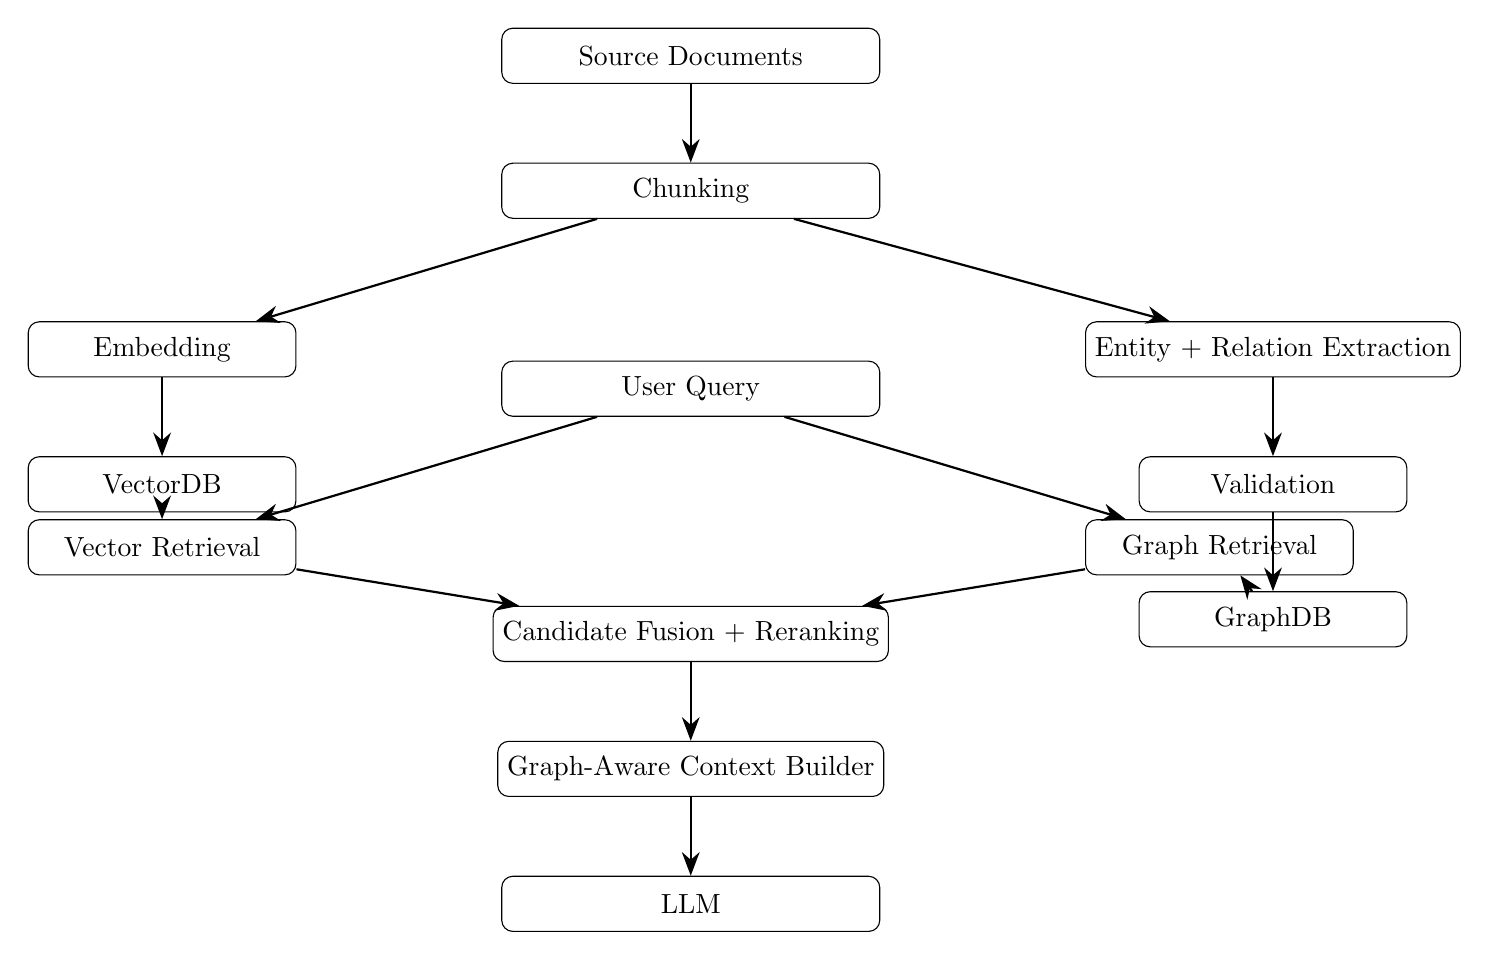
\begin{tikzpicture}[
node distance=1cm,
box/.style={draw,rounded corners,minimum width=4.8cm,minimum height=.7cm,align=center},
smallbox/.style={draw,rounded corners,minimum width=3.4cm,minimum height=.7cm,align=center},
arrow/.style={-{Stealth[length=3mm]},thick}
]
\node[box] (docs) {Source Documents};
\node[box,below=of docs] (chunks) {Chunking};

\node[smallbox,below left=1.3cm and 2.6cm of chunks] (emb) {Embedding};
\node[smallbox,below=of emb] (vdb) {VectorDB};

\node[smallbox,below right=1.3cm and 2.6cm of chunks] (extract) {Entity + Relation Extraction};
\node[smallbox,below=of extract] (valid) {Validation};
\node[smallbox,below=of valid] (gdb) {GraphDB};

\node[box,below=1.8cm of chunks] (query) {User Query};
\node[smallbox,below left=1.3cm and 2.6cm of query] (vr) {Vector Retrieval};
\node[smallbox,below right=1.3cm and 2.6cm of query] (gr) {Graph Retrieval};
\node[box,below=2.4cm of query] (fusion) {Candidate Fusion + Reranking};
\node[box,below=of fusion] (ctx) {Graph-Aware Context Builder};
\node[box,below=of ctx] (llm) {LLM};

\draw[arrow] (docs)--(chunks);
\draw[arrow] (chunks)--(emb);
\draw[arrow] (emb)--(vdb);
\draw[arrow] (chunks)--(extract);
\draw[arrow] (extract)--(valid);
\draw[arrow] (valid)--(gdb);

\draw[arrow] (query)--(vr);
\draw[arrow] (query)--(gr);
\draw[arrow] (vdb)--(vr);
\draw[arrow] (gdb)--(gr);
\draw[arrow] (vr)--(fusion);
\draw[arrow] (gr)--(fusion);
\draw[arrow] (fusion)--(ctx);
\draw[arrow] (ctx)--(llm);
\end{tikzpicture}
\end{center}

\section{Summary of Design Decisions}

The following design choices provide a clean reference implementation:

\begin{enumerate}
\item Store chunks and embeddings in the VectorDB.
\item Store entities and validated relationships in the GraphDB.
\item Keep ontology and extraction rules version-controlled outside the GraphDB.
\item Store entity IDs in vector metadata.
\item Store source chunk provenance on graph nodes or relationships.
\item Avoid automatically embedding the entire graph neighborhood into every chunk.
\item Perform graph traversal explicitly at inference time.
\item Support vector-first, graph-first, and parallel retrieval strategies.
\item Use candidate union and deduplication to combine retrieval outputs.
\item Apply reranking to select the strongest evidence.
\item Build final context from both relationship paths and source-backed textual evidence.
\item Evaluate Graph-RAG specifically on multi-hop, dependency, relationship, and impact queries.
\end{enumerate}

The central architectural principle is:

\begin{center}
\fbox{\parbox{0.85\textwidth}{
\centering
The VectorDB provides semantic evidence retrieval.\\
The GraphDB provides structural relationship retrieval.\\
Stable identifiers and provenance connect the two representations.\\
A retrieval orchestration layer determines how semantic and structural evidence are fused before context is supplied to the LLM.
}}
\end{center}

\end{document}
